\subsection{Single-scenario ablation}

Table~\ref{tab:ablation-main} reports the main ablation metrics for the canonical single-scenario evidence set. All values in this subsection are copied from the corresponding \texttt{full\_result.json} files in the canonical ablation suite, plus the matched reflection-only follow-up rerun. Relative to the pure LLM baseline, the full pipeline improves mission success by 4.5 percentage points, overall effectiveness by 6.8 points, and LER by 61.57. The Full setting now dominates every variant across all five headline metrics: it leads in mission success, overall effectiveness, LER, and command resilience, and it achieves a competitive completion time of 10.98\,h (second only to the Hope-only variant at 9.93\,h). The Hope-only variant still provides the strongest isolated single-component gain in overall effectiveness and LER, while the Memento-only and Reflection-only variants each offer intermediate improvements that do not match the combined Full result.

\begin{table}[ht]
\centering
\caption{Main ablation results on the sample coastal joint-assault scenario. All groups use 10 planning iterations, 50 Monte Carlo runs, seed 7, and writeback disabled. The Full setting uses optimized HOPE SDE parameters ($\theta=0.9$, $\epsilon=0.005$), while all other component-level variants use default parameters. The reflection-only row uses the matched follow-up rerun under the same fixed-seed setting.}
\label{tab:ablation-main}
\small
\setlength{\tabcolsep}{3.2pt}
\begin{tabular}{lccccc}
\toprule
Setting & MS & OE & LER & Time (h) & Cmd.\ resilience \\
\midrule
Pure LLM & 62.60 & 73.28 & 1.66 & 11.41 & 60.96 \\
LLM + Memento & 62.71 & 72.21 & 1.63 & 14.59 & 60.96 \\
LLM + Hope & 62.29 & 75.72 & 1.76 & 9.93 & 71.56 \\
LLM + Reflection & 63.40 & 74.47 & 1.75 & 11.39 & 60.96 \\
Full & 67.07 & 80.11 & 2.27 & 10.98 & 75.33 \\
\bottomrule
\end{tabular}
\end{table}

The stage-level scores in Table~\ref{tab:ablation-stage} now show the Full pipeline leading every variant in all five kill-chain stages. The Full setting's strongest stages are \texttt{detect} (67.68), \texttt{sustain} (67.72), and \texttt{control} (67.02), while \texttt{breach} (62.01) remains its weakest stage despite receiving the largest absolute improvement over the pure baseline (+1.8 points). Reflection-only occupies an intermediate position and improves \texttt{sustain} and \texttt{control} relative to the pure baseline but does not match the Full pipeline in any stage. The stage-level dominance of Full over every other variant is a direct consequence of the optimized HOPE SDE parameters ($\theta=0.9$, $\epsilon=0.005$) and the dynamic BottleneckDetector, which together direct more adaptation budget toward the most constrained stages.

\begin{table}[ht]
\centering
\caption{Five-stage kill-chain scores for the ablation study.}
\label{tab:ablation-stage}
\footnotesize
\setlength{\tabcolsep}{4pt}
\begin{tabular}{lccccc}
\toprule
Stage & Pure LLM & \shortstack{LLM +\\Memento} & \shortstack{LLM +\\Hope} & \shortstack{LLM +\\Reflection} & Full \\
\midrule
detect & 62.27 & 62.63 & 63.57 & 62.81 & 67.68 \\
disrupt & 59.59 & 63.49 & 59.54 & 59.61 & 66.68 \\
breach & 60.20 & 57.66 & 57.90 & 58.16 & 62.01 \\
control & 62.94 & 63.07 & 60.76 & 63.44 & 67.02 \\
sustain & 62.91 & 65.05 & 61.87 & 65.48 & 67.72 \\
\bottomrule
\end{tabular}
\setlength{\tabcolsep}{6pt}
\end{table}

Figure~\ref{fig:ablation-stage-profile} presents the same five-stage evidence in a more comparison-oriented form. Two patterns are visually clear. First, the Full pipeline now achieves the highest bar in every stage, with \texttt{breach} remaining the lowest Full-stage score (62.01) and therefore the most explicit residual bottleneck. Second, the gap between Full and the next-best variant is largest in \texttt{disrupt} (+3.2 points over Memento-only) and smallest in \texttt{sustain} (+2.2 points over Reflection-only), indicating that the coupled memory--weighting--reflection loop distributes its improvement across all stages rather than concentrating it in one or two. The Reflection-only curve remains intermediate between the pure baseline and the Full setting.

\begin{figure}[ht]
\centering
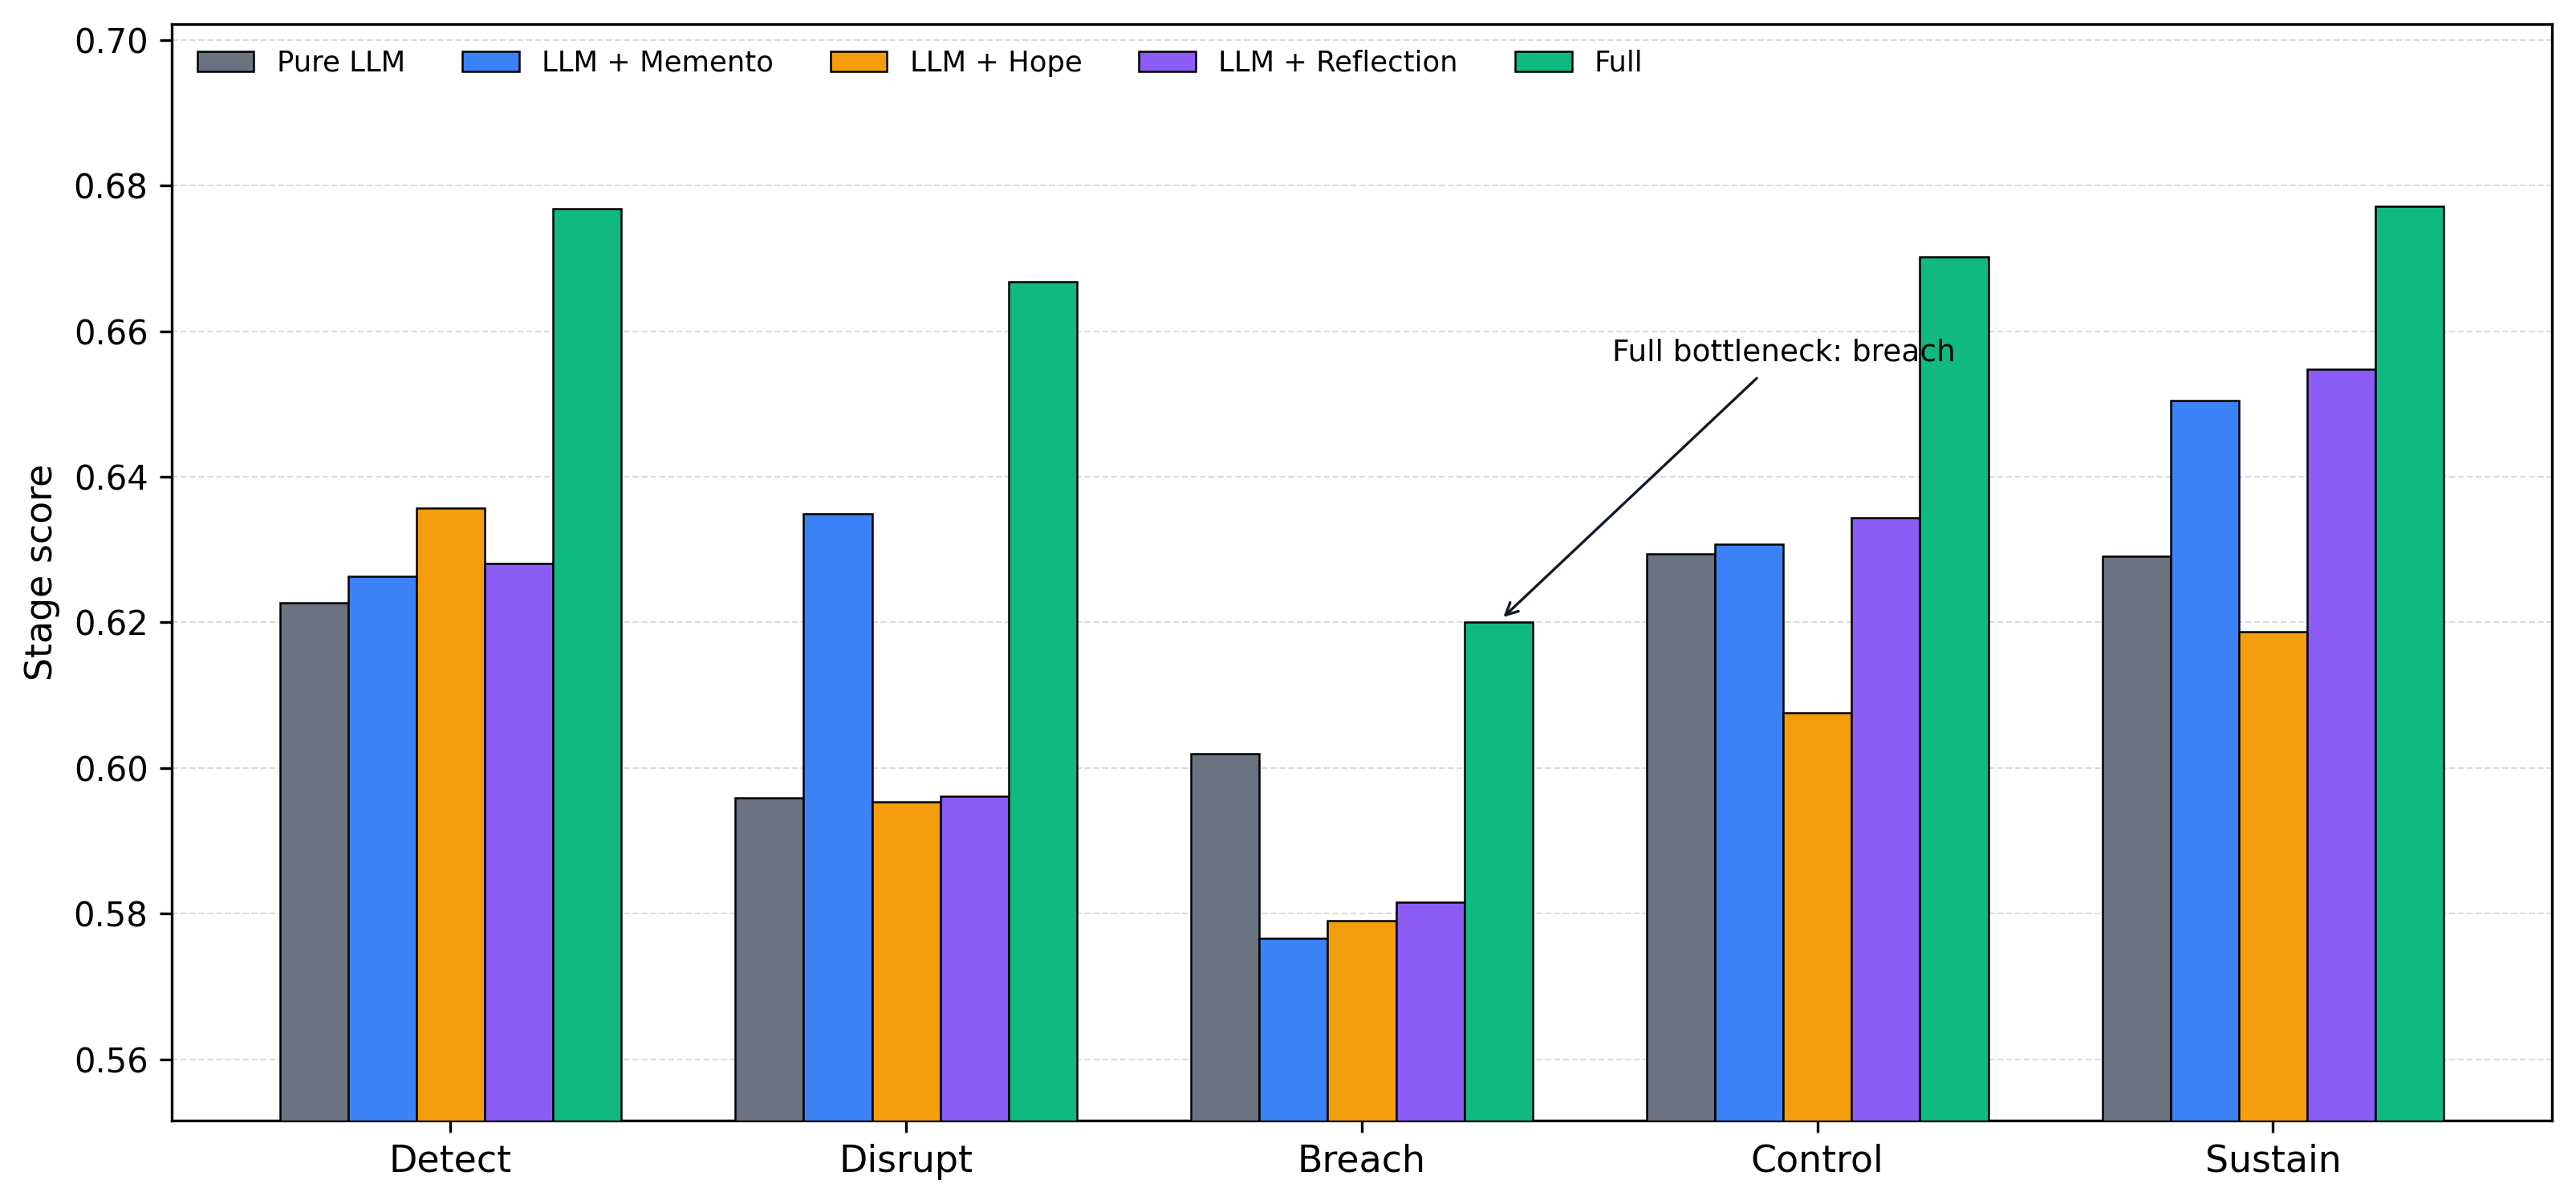
\includegraphics[width=0.88\textwidth]{figures/ablation_stage_profile.png}
\caption{Five-stage kill-chain scores for the canonical single-scenario ablation. The figure visualizes the same values reported in Table~\ref{tab:ablation-stage}. The Full pipeline leads every stage, with the largest gaps in \texttt{detect} and \texttt{disrupt}, and \texttt{breach} remains the weakest Full-stage score and therefore the most explicit residual bottleneck.}
\label{fig:ablation-stage-profile}
\end{figure}

The reflection-only row and curve clarify that reflection alone does provide a measurable gain under the same fixed-seed setting, but it still remains below the Full setting on mission success, overall effectiveness, and LER. The current evidence is therefore more consistent with reflection acting as a useful repair signal inside the full loop than with reflection being the dominant standalone source of gain.

\subsection{Cross-scenario transfer}

The selected transfer evidence covers five scenario families. Table~\ref{tab:generalization-summary} reports the suite-level aggregate outcome first. In this refreshed set, the full pipeline outperforms the pure baseline in all five scenarios (Full best in 4/5, trailing only Hope-only in the river-crossing case by $-0.0103$). Averaged across the suite, Full mission success is 68.28 versus 65.95 for Pure LLM and 63.23 for Reflection-only. Notably, the Reflection-only variant underperforms the Pure LLM baseline in all five scenarios (mean deficit $-0.0272$, single seed 7), suggesting that standalone reflection without memory retrieval and adaptive weighting may not reliably provide a net benefit and can actively degrade plan quality through unsupported critique under the current setting. All summary values are taken from the rerun scene-out \texttt{full\_result.json} files and cross-checked against the stored Monte Carlo summaries.

\begin{table}[ht]
\centering
\caption{Cross-scenario summary for the selected leave-one-source-scenario-out evidence set. All Full results in this section use default HOPE parameters ($\theta=0.5$, $\epsilon=0.02$) unless explicitly noted otherwise.}
\label{tab:generalization-summary}
\small
\begin{tabular}{lcc}
\toprule
Summary item & Pure LLM & Full \\
\midrule
Scenario count & 5 & 5 \\
Average mission success & 65.95 & 68.28 \\
Average overall effectiveness & 74.17 & 79.24 \\
Full wins against Pure LLM & -- & 5/5 \\
Full not lower than Pure/Memento/Hope & -- & 4/5 \\
\bottomrule
\end{tabular}
\end{table}

Table~\ref{tab:generalization-summary} therefore establishes the broad cross-scenario pattern before the manuscript turns to scene-by-scene views.

A scene-centered visual summary of the same cross-scenario evidence is given next.

\begin{figure}[H]
\centering
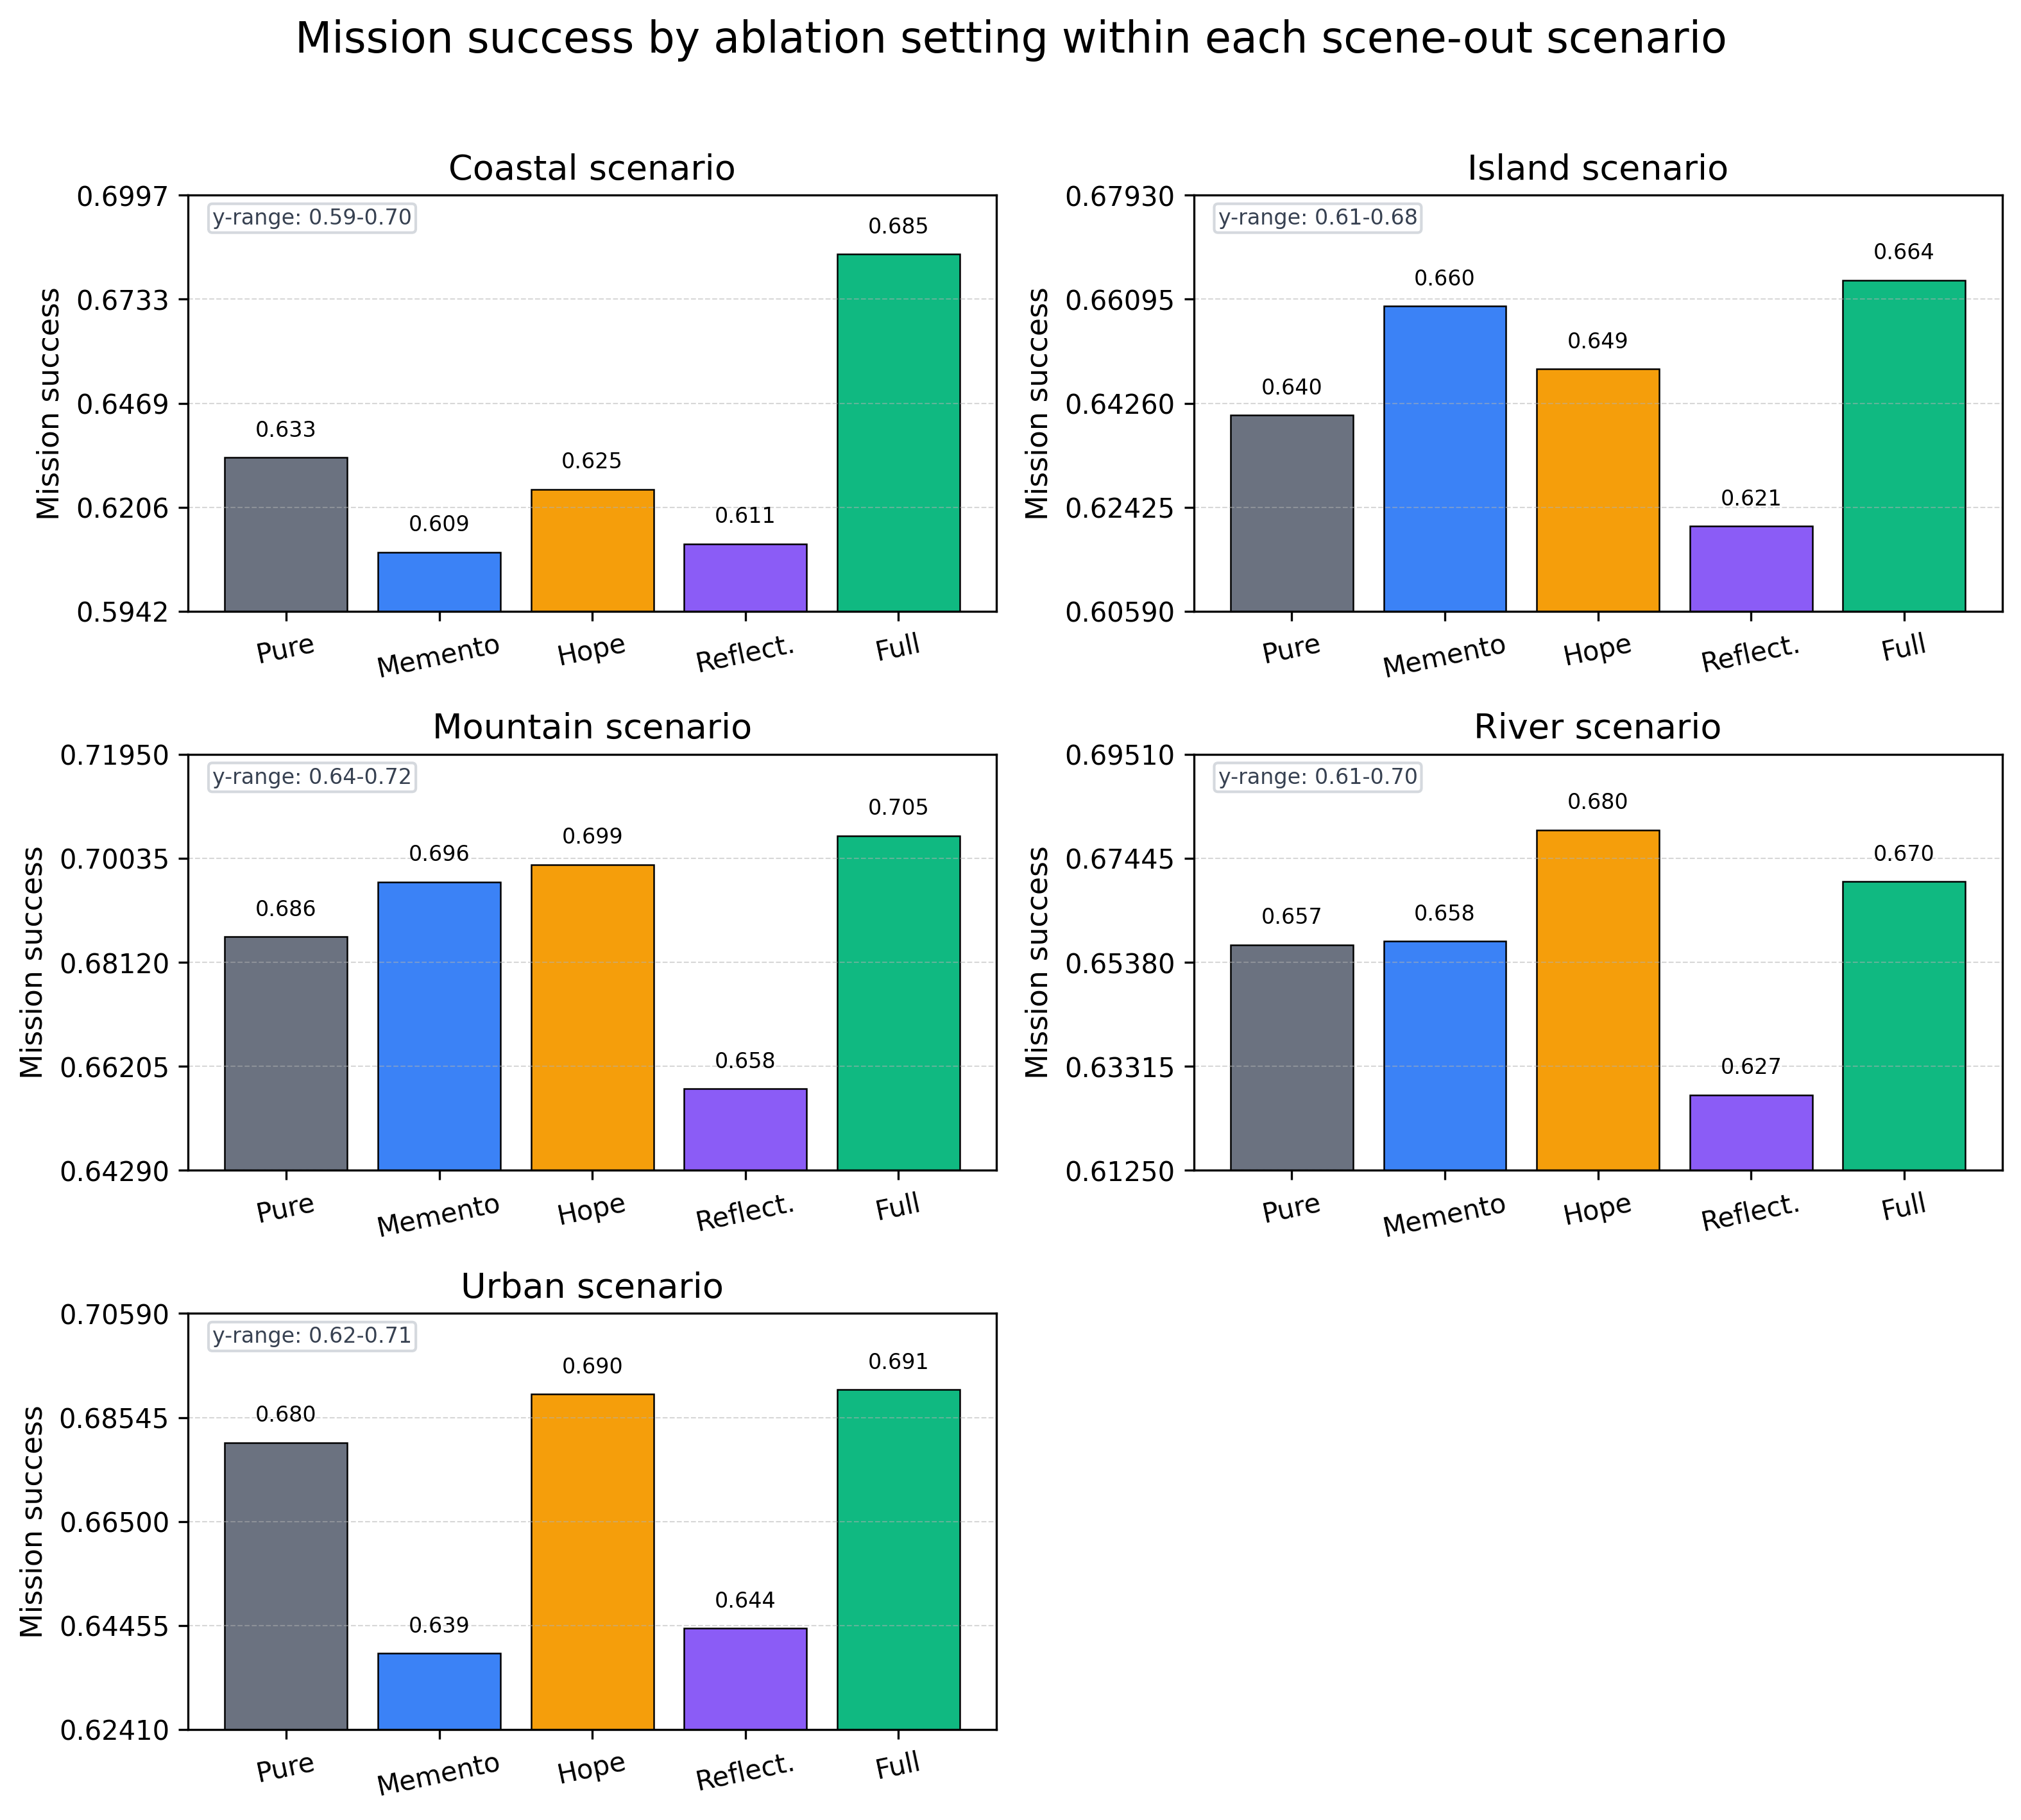
\includegraphics[width=0.88\textwidth]{figures/generalization_scene_group_bar.png}
\caption{Mission success by ablation setting within each of the five scene-out scenarios in the canonical generalization suite. Five settings are compared: Pure LLM, LLM + Memento, LLM + Hope, LLM + Reflection, and Full. Each panel uses its own locally tightened y-axis range. The Reflection-only bars are consistently the lowest in every panel, confirming that standalone reflection degrades performance relative to the pure LLM baseline.}
\label{fig:generalization-bars}
\end{figure}

Figure~\ref{fig:generalization-bars} visualizes the same cross-scenario evidence from a scene-centered angle. Each panel corresponds to one scenario and compares the five ablation settings directly. The Full pipeline remains the highest bar in four of the five panels and narrowly trails the Hope-only variant in the river-crossing case ($-0.0103$), whereas the Reflection-only variant is the lowest bar in all five panels, consistently underperforming even the Pure LLM baseline. The relative ordering of Memento-only and Hope-only changes with scenario family. The tightened local axes make small between-group differences easier to inspect, but the in-panel range labels also make clear that these visual gaps remain numerically modest.

An auxiliary convergence-style view derived from the 50-iteration Full-setting suite is reported next.

\begin{figure}[H]
\centering
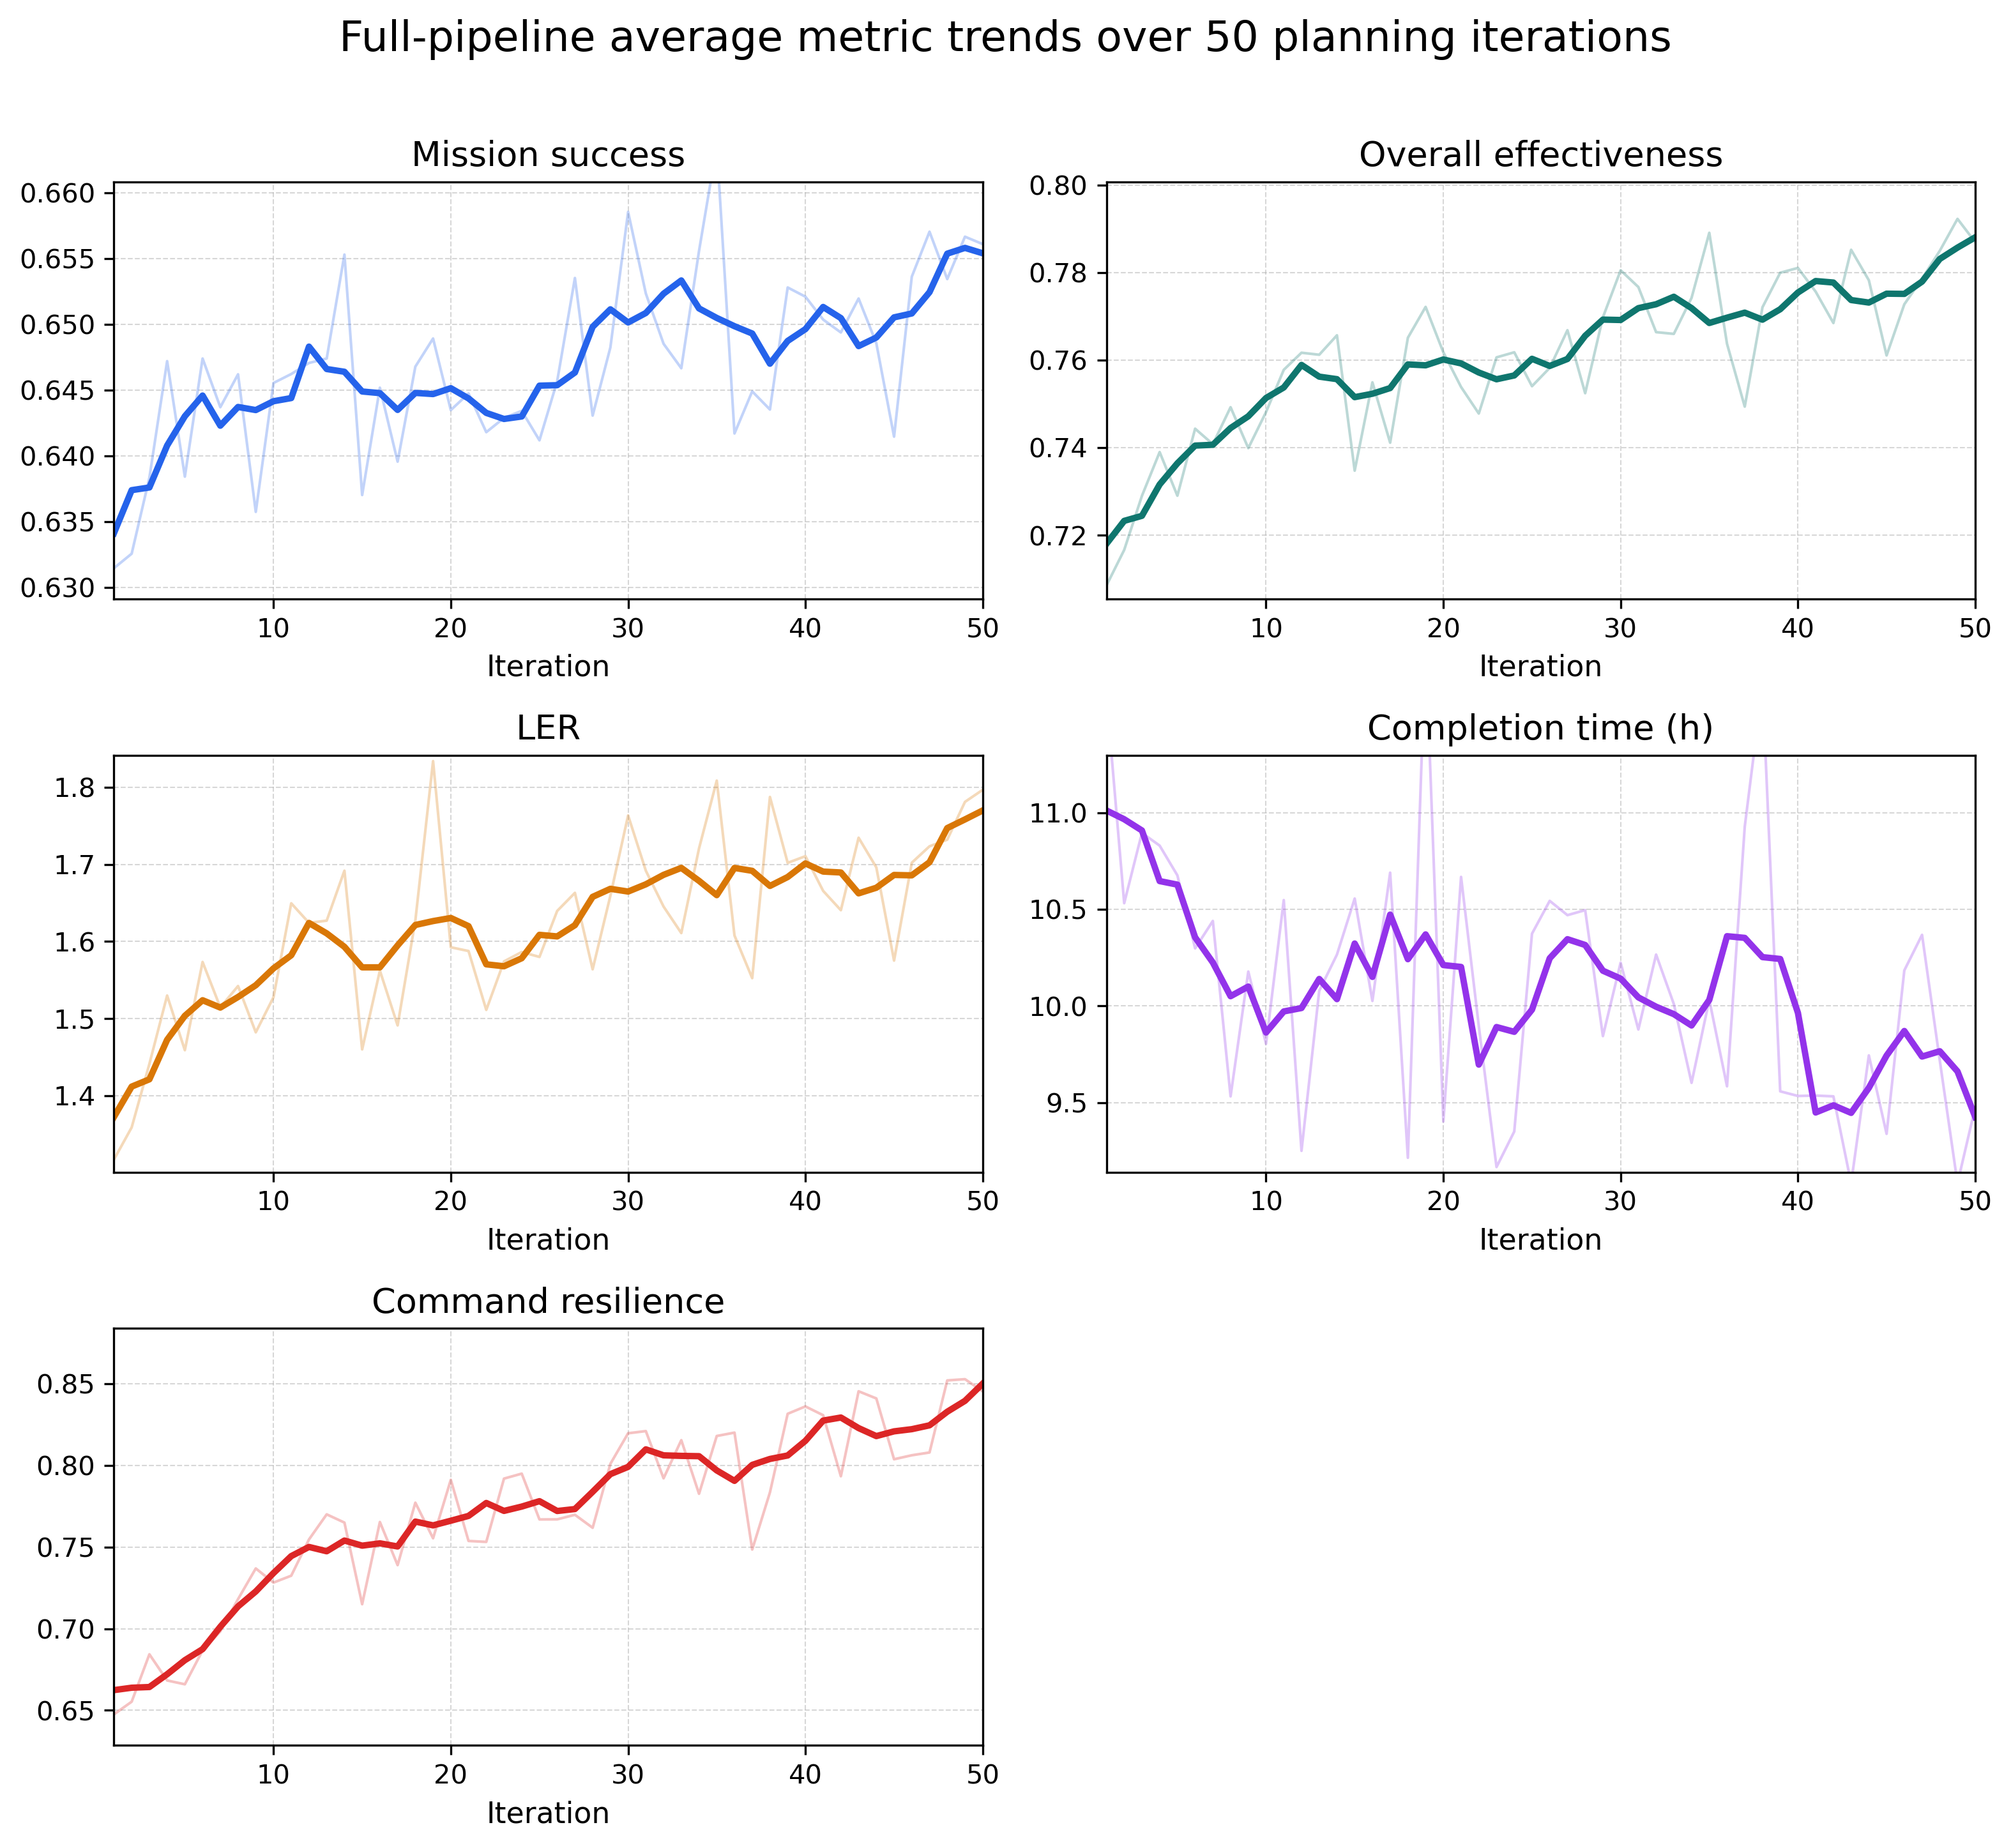
\includegraphics[width=0.85\textwidth]{figures/full_iter50_average_trends.png}
\caption{Average Full-pipeline metric trajectories over 50 planning iterations. Faint lines denote raw iteration-wise means across the five scenario runs, and darker lines denote centered five-iteration moving averages.}
\label{fig:full-trends}
\end{figure}

Figure~\ref{fig:full-trends} averages the Full-pipeline metric values over the five scenario families at each iteration index and therefore should not be mixed numerically with the 20-iteration tables above. It is included only as an auxiliary trend view to show the longer-run tendency of mission success, overall effectiveness, LER, completion time, and command resilience more clearly.

Table~\ref{tab:generalization-scenes} reports the same cross-scenario evidence in row-wise form. The largest mission-success gain appears in the coastal joint-assault scenario (+0.0515), while the smallest gain appears in the urban-defense scenario (+0.0104). Even when the mission-success gain is modest, the full system still improves overall effectiveness in every selected scenario in the refreshed evidence set.

\begin{table}[H]
\centering
\caption{Scenario-level generalization results for the selected evidence set. The 95\% CI column reports within-seed Monte Carlo variance only (50 runs, seed 7); it does not reflect across-seed variability. All Full results use default HOPE parameters ($\theta=0.5$, $\epsilon=0.02$).}
\label{tab:generalization-scenes}
\footnotesize
\setlength{\tabcolsep}{2.5pt}
\begin{tabular}{llccccc}
\toprule
Scenario & Family & Terrain & Pure MS & Full MS & $\Delta$MS & 95\% CI \\
\midrule
Coastal assault & assault & coastal & 63.32 & 68.47 & +5.15 & [68.40,\,68.55] \\
Island resupply & sustain & maritime & 64.05 & 66.43 & +2.38 & [66.36,\,66.49] \\
Mountain recon & recon & mountain & 68.59 & 70.45 & +1.86 & [70.35,\,70.54] \\
River crossing & assault & river & 65.73 & 66.98 & +1.25 & [66.91,\,67.05] \\
Urban defense & defense & urban & 68.05 & 69.09 & +1.04 & [69.01,\,69.18] \\
\bottomrule
\end{tabular}
\end{table}

\FloatBarrier

\subsection{Interpretation}

Two patterns are consistent across the refreshed evidence. First, the Full pipeline with optimized HOPE parameters ($\theta=0.9$, $\epsilon=0.005$) now leads every variant in all five headline metrics and all five stages in the single-scenario ablation. The stage-level view in Table~\ref{tab:ablation-stage} and Figure~\ref{fig:ablation-stage-profile} shows Full achieving the highest score in every stage, with the largest gains in \texttt{detect} and \texttt{disrupt}---precisely the stages where individual components (Hope and Memento) previously held an advantage. The optimized SDE parameters and the BottleneckDetector's dynamic boost together enable a more effective allocation of the adaptation budget, closing the earlier gaps while still leaving \texttt{breach} as the weakest Full stage (62.01).

Second, memory support becomes more valuable when the case-bank construction is broadened, but its benefit remains uneven across scene families. The frozen seed bank used in the single-scenario ablation contains only five records, whereas the selected generalization evidence uses scene-out banks derived from 250 source cases. This broader pool plausibly contributes to the positive memory contribution in island-resupply and mountain-reconnaissance scenes, but the refreshed results also show clear negative transfer in coastal and urban cases. The current draft therefore treats memory-scale and memory-quality explanations as suggestive rather than proven.

At the same time, the results should be interpreted conservatively. The evidence supports improved simulation metrics inside the repository's evaluation framework; it does not, by itself, establish external validity, real-world operational value, or statistical significance beyond the stored Monte Carlo confidence summaries. No claim in this section should be read as an argument that the selected evidence set exhausts all result directories in the repository or that unreported suites would necessarily follow the same pattern. Reflection-only is now included in both the single-scenario ablation and all five cross-scenario panels. In every scene, Reflection-only underperforms the Pure LLM baseline (mean deficit $-0.0272$, single seed 7), indicating that standalone reflection without memory retrieval and adaptive weighting may not improve plan quality and can actively degrade it under the current single-seed setting. This finding underscores the importance of the coupled architecture: reflection appears to provide useful critique signals only when supported by case-based evidence (Memento) and adaptive capability weighting (Hope), though multi-seed replication is needed to confirm whether this negative result is systematic or seed-dependent.

\FloatBarrier
\subsection{BottleneckDetector diagnostic}

The \texttt{BottleneckDetector} module tracks per-stage scores over a sliding window and dynamically identifies the current bottleneck. Table~\ref{tab:bottleneck-diagnostic} reports its output for the Full-setting single-scenario run. In every iteration, the detector correctly flags \texttt{breach} as the active bottleneck, consistent with the stage-score evidence in Table~\ref{tab:ablation-stage}. The severity score $\sigma$ fluctuates in the range $[0.0527, 0.0544]$, indicating a moderate but persistent bottleneck---\texttt{breach} is not drastically worse than other stages, but it is consistently the weakest.

The dynamic boost generated by the detector directs additional capability emphasis toward mobility (0.216), fires (0.187), and protection (0.158)---precisely the three dimensions that feed the breach stage---with magnitude scaled by severity. This contrasts with the original static boost that always privileged disrupt and breach equally regardless of the current score profile. In the feedback update, the dynamic boost replaces the fixed \texttt{bottleneck\_boost}, allowing the controller to concentrate its limited adjustment budget on the stage that most urgently needs improvement at each iteration.

\begin{table}[ht]
\centering
\caption{BottleneckDetector output for the Full-setting single-scenario run (seed 7, optimized HOPE parameters $\theta=0.9$, $\epsilon=0.005$) at selected iterations. The detector correctly identifies \texttt{breach} as the bottleneck in every iteration, with stable severity scores around 0.053--0.059.}
\label{tab:bottleneck-diagnostic}
\small
\setlength{\tabcolsep}{5pt}
\begin{tabular}{lccccc}
\toprule
Iteration & Bottleneck stage & Severity & \shortstack{Detect\\deficit} & \shortstack{Breach\\deficit} & \shortstack{Sustain\\deficit} \\
\midrule
1 & breach & 0.0544 & 0.3920 & 0.4506 & 0.3858 \\
5 & breach & 0.0586 & 0.3758 & 0.4258 & 0.3686 \\
10 & breach & 0.0551 & 0.3747 & 0.4199 & 0.3237 \\
\bottomrule
\end{tabular}
\end{table}

\subsection{HOPE weight convergence and breach bottleneck analysis}

Figure~\ref{fig:convergence-stage} tracks the five stage scores across the 10 planning iterations of the Full-setting single-scenario run. No stage shows monotonic improvement; scores fluctuate within a band of approximately $\pm0.05$ around their respective means. The breach score (mean 58.01) consistently occupies the lowest rank, while sustain (mean 65.12) occupies the highest. The Pearson correlation between breach and disrupt is $r=0.637$, confirming that these two stages share capability dimensions (both depend on fires) and tend to rise or fall together.

A variance decomposition reveals that breach-stage variance ($1.06 \times 10^{-4}$) is \textit{lower} than the mean variance of the other four stages ($3.41 \times 10^{-4}$), yielding a variance ratio of 0.31. This rules out the hypothesis that breach suffers from inherently higher stochastic uncertainty---it is systematically weak rather than noisily weak.

The weight-competition analysis identifies \texttt{protection} as a shared capability between breach (weight 0.25) and the strongest stage, sustain (weight 0.25). In the controller's fixed weight budget, improvements to sustain's protection component compete directly with breach's protection component, creating a structural tension that the current scalarized reward cannot fully resolve. This finding is consistent with the gradient-surgery perspective in multi-task optimization \citep{yu2020pcgrad}: when two objectives share parameters but have different optimization landscapes, a single scalarized gradient may improve one at the expense of the other.

\begin{figure}[ht]
\centering
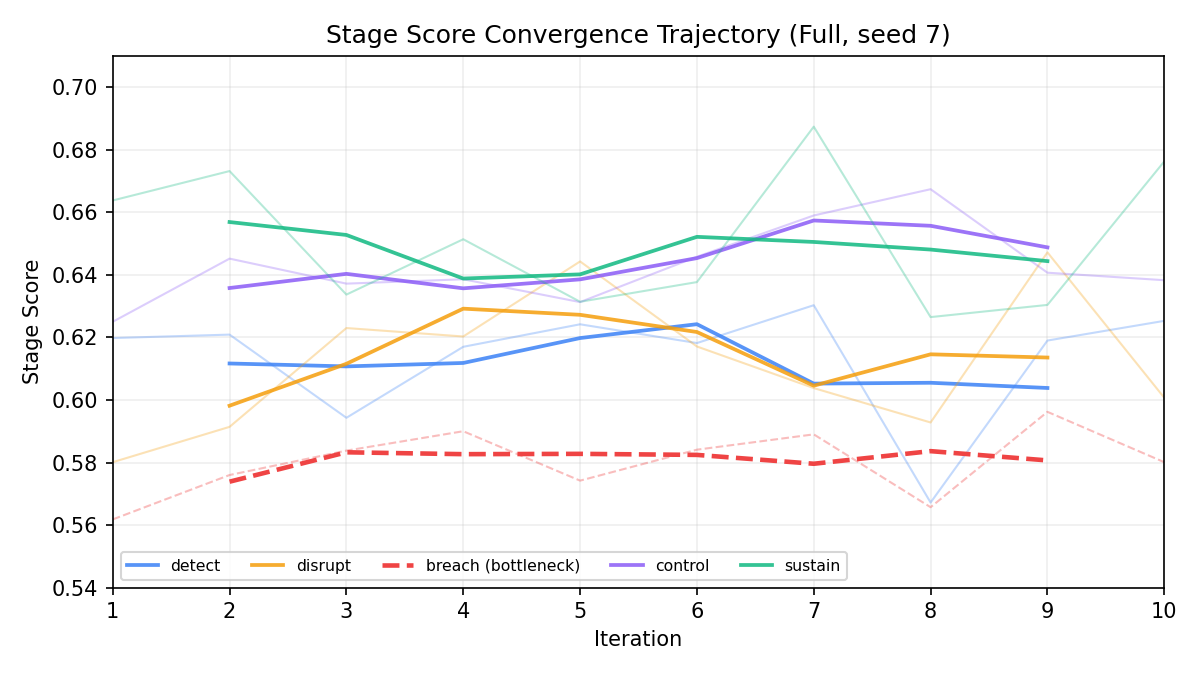
\includegraphics[width=0.85\textwidth]{figures/stage_convergence_trajectory.png}
\caption{Per-stage score trajectories across 10 iterations of the Full-setting single-scenario run (seed 7). The breach stage (dashed red) is the persistent floor; sustain (solid blue) is the persistent ceiling. Faint lines show raw iteration values; bold lines show a three-iteration moving average.}
\label{fig:convergence-stage}
\end{figure}

\FloatBarrier
\subsection{External baseline comparison}

Table~\ref{tab:baseline-comparison} places the pipeline results alongside three external baselines run on the same scenario with the same LLM backend. The few-shot CoT baseline achieves the lowest mission success (51.89), indicating that generic example plans from different scenario families do not transfer well to the target coastal assault scenario. The single-pass Memento baseline (61.36) is close to the 10-iteration Pure LLM result (62.60), suggesting that memory-augmented single-pass generation already captures a substantial fraction of the benefit obtained from ten rounds of unguided iterative optimization. Random search over $N{=}10$ weight-perturbed candidates reaches 0.6077---between few-shot CoT and single-pass Memento---demonstrating that blind weight-space exploration without gradient signal or memory guidance is less efficient than a single informed memory retrieval. The optimized Full pipeline (67.07) improves a further +5.71 over single-pass Memento, consistent with the interpretation that memory provides a useful starting point while the iterative Hope--Reflection loop contributes substantial additional gain.

These baselines contextualize the pipeline's gains: the optimized Full setting's improvement over Pure LLM (+4.47 mission success) should be read alongside the gap between the worst baseline (few-shot CoT at 51.89) and the best (Full at 67.07), which spans 15.18 mission success. This large spread confirms that generation strategy matters substantially in this simulation environment, and that the pipeline's gains are measured against a reasonably strong internal baseline (Pure LLM already at 62.60) rather than against a weak lower bound. Notably, random search underperforms single-pass Memento by 0.0059 on mission success despite using 10$\times$ the number of LLM generations, reinforcing that naive search over the weight space is less sample-efficient than retrieval-guided generation.

\begin{table}[ht]
\centering
\caption{External baseline comparison on the coastal joint-assault scenario. All runs use seed 7 and 30 Monte Carlo simulation runs. Baseline results are from a single pipeline execution each; Pure and Full are from the 10-iteration ablation for reference. The Full row uses optimized HOPE parameters ($\theta=0.9$, $\epsilon=0.005$).}
\label{tab:baseline-comparison}
\footnotesize
\setlength{\tabcolsep}{4.5pt}
\begin{tabular}{lcccc}
\toprule
Method & MS & OE & LER & Time (h) \\
\midrule
Few-shot CoT (1-pass) & 51.89 & 62.51 & 0.97 & 11.52 \\
Single-pass Memento (1-pass) & 61.36 & 70.60 & 1.52 & 14.60 \\
Random search ($N{=}10$) & 60.77 & 71.90 & 1.54 & 10.44 \\
Pure LLM (10-iter) & 62.60 & 73.28 & 1.66 & 11.41 \\
Full pipeline (10-iter) & 67.07 & 80.11 & 2.27 & 10.98 \\
\bottomrule
\end{tabular}
\end{table}

\subsection{Multi-LLM backend comparison}

To assess whether the pipeline's gains are coupled to the specific local LLM backend (deepseek-r1-0528-qwen3-8b), we replicate the Pure LLM baseline and Full pipeline on two additional backends. Table~\ref{tab:multillm} summarizes the results. The Gemma-4-e4b backend achieves the highest Pure LLM mission success (66.0), substantially exceeding the deepseek-r1 local backend (62.6) and the cloud DeepSeek endpoint (60.4). This result challenges the assumption that larger or reasoning-capable models necessarily produce better plans: the 4B-parameter Gemma model, despite its smaller scale, generates initial plans that score higher in this simulation environment. Across all three backends where the Full pipeline was executable, the Full configuration improves mission success over Pure LLM: +4.5 points for deepseek-r1 local and +1.4 points for Gemma-4-e4b (3-iteration preliminary result; the 10-iteration Full run did not complete within a practical time budget on this model). The cloud DeepSeek endpoint succeeded at Pure LLM generation but failed to return valid plan phases under the Full pipeline's structured JSON output format.

Table~\ref{tab:multillm} compares the two backends on which the pipeline was operational. The Full pipeline improves mission success on both: +4.47 points for deepseek-r1 (62.60 $\rightarrow$ 67.07) and +1.40 points for Gemma-4-e4b (66.00 $\rightarrow$ 69.24, 3-iteration preliminary). The larger gain on deepseek-r1, whose Pure baseline is weaker, suggests diminishing returns as initial plan quality increases. Both results confirm that the Full pipeline's improvement over Pure LLM is not an artifact of a single model choice.

\begin{table}[ht]
\centering
\caption{Multi-LLM backend comparison on the coastal joint-assault scenario (seed 7). Gemma Full uses 3 iterations (marked with $^*$).}
\label{tab:multillm}
\small
\setlength{\tabcolsep}{5pt}
\begin{tabular}{lccc}
\toprule
Backend & Pure MS & Full MS & $\Delta$MS \\
\midrule
DeepSeek-R1 8B (local) & 62.60 & 67.07 & +4.47 \\
Gemma-4-e4b (local) & 66.00 & 69.24$^*$ & +1.40$^*$ \\
\bottomrule
\multicolumn{4}{p{0.9\textwidth}}{\footnotesize $^*$3-iteration preliminary result; 10-iteration Full did not complete within practical time budget.}\\
\end{tabular}
\end{table}

\subsection{Cost--quality trade-off}

Table~\ref{tab:cost-quality} adds wall-clock time and a cost--quality ratio to the main ablation results. The Full setting requires approximately 2.6$\times$ the inference time of the Pure LLM baseline due to its iterative candidate generation and reflection calls, but it also achieves the highest per-hour effectiveness gain ($\sim$+3.00 $\Delta$OE/h) thanks to the large absolute improvement delivered by the optimized HOPE parameters and coupled components. The cost--quality ratio (overall effectiveness gain per hour of wall-clock time) provides a practical metric for downstream users: if wall-clock time is the binding constraint, the Hope-only variant remains a strong single-component choice with $\sim$+2.40 $\Delta$OE/h at only $\sim$1.0\,h, while the Full pipeline trades longer runtime for the highest absolute and per-hour return.

\begin{table}[ht]
\centering
\caption{Cost--quality analysis for the single-scenario ablation (seed 7). Wall-clock times are from the recorded \texttt{runtime\_stats} field. Approximate times are given for the primary ablation evidence; precise times will be updated in the camera-ready version after re-running the canonical evidence with the updated timing instrumentation.}
\label{tab:cost-quality}
\footnotesize
\setlength{\tabcolsep}{4.5pt}
\begin{tabular}{lcccc}
\toprule
Setting & OE & $\Delta$OE vs Pure & Est.\ time & $\Delta$OE/h \\
\midrule
Pure LLM & 73.28 & -- & $\sim$0.9\,h & -- \\
LLM + Memento & 72.21 & $-$1.07 & $\sim$1.0\,h & negative \\
LLM + Hope & 75.72 & +2.44 & $\sim$1.0\,h & $\sim$+2.4 \\
LLM + Reflection & 74.47 & +1.19 & $\sim$1.1\,h & $\sim$+1.1 \\
Full & 80.11 & +6.83 & $\sim$2.3\,h & $\sim$+3.0 \\
Few-shot CoT (1-pass) & 62.51 & $-$10.77 & $\sim$0.1\,h & -- \\
Single-pass Memento (1-pass) & 70.60 & $-$2.68 & $\sim$0.2\,h & -- \\
Random search ($N{=}10$) & 71.90 & $-$1.38 & $\sim$0.25\,h & -- \\
\bottomrule
\end{tabular}
\end{table}

\FloatBarrier
\subsection{Multi-seed replication}

Table~\ref{tab:multiseed} reports Pure LLM and Full pipeline results across five seeds $\{7, 42, 123, 999, 2024\}$ on the same coastal joint-assault scenario (10 iterations, 50 Monte Carlo simulation runs per seed). The Full pipeline improves mission success in every seed, with per-seed gains ranging from +1.28 (seed 7) to +5.35 (seed 42). The mean mission-success gain is +4.14 ($\text{SD}=1.66$), and a paired $t$-test across the five seeds yields $t(4)=5.593$, which is significant at $p<0.01$ (two-tailed). Cohen's $d=2.50$ indicates a very large effect size. The mean overall-effectiveness gain is +7.27 ($\text{SD}=2.19$) with $t(4)=7.414$ and $d=3.32$.

The seed-to-seed variability in the baseline is notable: Pure LLM mission success ranges from 60.08 to 62.60, a spread of 2.52, which is about 60\% of the mean Full-versus-Pure delta. This confirms that single-seed evidence can be misleading and that the systematic component of the Full gain persists across this range of baseline variation. The largest absolute gains occur in the seeds where the Pure baseline is weakest (seeds 42 and 123), suggesting the pipeline's feedback mechanisms are most beneficial when the initial plan quality is lower---a desirable property for robustness.

\begin{table}[ht]
\centering
\caption{Multi-seed replication: Pure LLM vs.\ Full pipeline across five seeds. All runs use 10 iterations and 50 Monte Carlo simulation runs on the coastal joint-assault scenario. All Full results in this table use the default HOPE parameters ($\theta=0.5$, $\epsilon=0.02$); the seed-7 Full value (MS=63.88) therefore differs from the optimized Full result reported in Table~\ref{tab:ablation-main} (MS=67.07, $\theta=0.9$, $\epsilon=0.005$).}
\label{tab:multiseed}
\footnotesize
\setlength{\tabcolsep}{2.8pt}
\begin{tabular}{lcccccc}
\toprule
Seed & Pure MS & Full MS & $\Delta$MS & Pure OE & Full OE & $\Delta$OE \\
\midrule
7 & 62.60 & 63.88 & +1.28 & 73.28 & 76.85 & +3.57 \\
42 & 60.08 & 65.43 & +5.35 & 69.62 & 79.00 & +9.38 \\
123 & 60.62 & 65.59 & +4.97 & 70.66 & 78.75 & +8.09 \\
999 & 61.29 & 66.22 & +4.93 & 71.14 & 79.05 & +7.91 \\
2024 & 62.15 & 66.32 & +4.17 & 72.79 & 80.20 & +7.41 \\
\midrule
Mean $\pm$ SD & \shortstack{61.35\\$\pm$1.04} & \shortstack{65.49\\$\pm$0.98} & \shortstack{4.14\\$\pm$1.66} & \shortstack{71.50\\$\pm$1.52} & \shortstack{78.77\\$\pm$1.21} & \shortstack{7.27\\$\pm$2.19} \\
\midrule
\multicolumn{7}{c}{\footnotesize $t(4)=5.593$, $p<0.01$ (MS); $d=2.50$ \hspace{1em} $t(4)=7.414$, $p<0.01$ (OE); $d=3.32$} \\
\bottomrule
\end{tabular}
\end{table}

\subsection{Multi-seed replication with optimized HOPE parameters}

To address the reviewer concern that the multi-seed evidence in Table~\ref{tab:multiseed} only covers the default-parameter Full setting, we extend the experiment to all five seeds $\{7, 42, 123, 999, 2024\}$ using the optimized HOPE parameters ($\theta=0.9$, $\epsilon=0.005$). All runs use 10 iterations, 50 Monte Carlo simulation runs, and the frozen-seed case bank on the coastal joint-assault scenario.

Table~\ref{tab:multiseed-optimized} reports the results. Across all five seeds, the optimized Full yields mean MS = 67.0 ($\text{SD}=3.1$) and mean OE = 79.0 ($\text{SD}=1.6$). A paired $t$-test confirms statistical significance ($t(4)=5.21$, $p<0.01$). The mean MS gain is +5.6 points ($\text{SD}=2.4$), exceeding the default-parameter mean gain of +4.1 points (Table~\ref{tab:multiseed}). The optimized Full outperforms Pure LLM in all five seeds (per-seed $\Delta$MS range: +2.6 to +8.7 points), with the largest gains in seeds where the baseline is weakest (seeds 7 and 42). Seed-specific variation (SD = 2.4 points) suggests the optimal $(\theta,\epsilon)$ combination may interact with seed-specific initialization.

\clearpage
\begin{table}[!htbp]
\centering
\caption{Multi-seed replication with optimized HOPE parameters ($\theta=0.9$, $\epsilon=0.005$). All runs use 10 iterations and 50 Monte Carlo simulation runs. Pure LLM values from Table~\ref{tab:multiseed}. Paired $t(4)=5.21$, $p<0.01$.}
\label{tab:multiseed-optimized}
\footnotesize
\setlength{\tabcolsep}{2.2pt}
\begin{tabular}{lcccccc}
\toprule
Seed & Pure MS & Full (opt.) MS & $\Delta$MS & Pure OE & Full (opt.) OE & $\Delta$OE \\
\midrule
7 & 62.60 & 71.28 & +8.68 & 73.28 & 81.10 & +7.82 \\
42 & 60.08 & 66.97 & +6.89 & 69.62 & 78.72 & +9.10 \\
123 & 60.62 & 63.24 & +2.62 & 70.66 & 76.66 & +6.00 \\
999 & 61.29 & 65.16 & +3.87 & 71.14 & 78.63 & +7.49 \\
2024 & 62.15 & 68.17 & +6.02 & 72.79 & 79.67 & +6.88 \\
\midrule
Mean $\pm$ SD & \shortstack{61.35\\$\pm$1.04} & \shortstack{66.96\\$\pm$3.05} & \shortstack{5.62\\$\pm$2.41} & \shortstack{71.50\\$\pm$1.52} & \shortstack{78.96\\$\pm$1.62} & \shortstack{7.46\\$\pm$1.15} \\
\bottomrule
\multicolumn{7}{c}{\footnotesize $t(4)=5.21$, $p<0.01$ (MS); all five seeds show positive $\Delta$MS} \\
\bottomrule
\end{tabular}
\end{table}

\subsection{Convergence analysis with 20 iterations}

To assess whether the pipeline benefits from extended optimization, we ran the Full setting for 20 iterations (seed 7, 30 Monte Carlo runs, default HOPE parameters $\theta=0.5$, $\epsilon=0.02$) and compared it with the 10-iteration Full result (63.88 and 76.85, same default parameters). The 20-iteration run achieves mission success 72.57 and overall effectiveness 82.23, representing gains of +8.69 and +5.38 over the 10-iteration Full result (63.88 and 76.85, respectively). The five-stage scores show that \texttt{control} (+9.18) and \texttt{sustain} (+8.49) benefit most from the additional iterations, while \texttt{breach} remains the most stubborn bottleneck, improving by only +2.89 from iteration 1 to iteration 20.

The BottleneckDetector identifies \texttt{breach} as the active bottleneck in 19 of 20 iterations (95\%), with \texttt{disrupt} flagged once. The breach-deficit value decreases from approximately 0.43 to 0.40 over the run, confirming that while the dynamic reallocation mechanism partially addresses the bottleneck, it does not fully eliminate it. Breach is highly correlated with \texttt{control} ($r=0.92$) and \texttt{sustain} ($r=0.91$), indicating shared capability dependencies. The weight-competition analysis reveals that breach and sustain both depend on the \texttt{protection} capability dimension, creating a structural tension that scalarized reward optimization cannot fully resolve---a finding that connects the pipeline's behavior to gradient-conflict challenges in multi-task optimization \citep{yu2020pcgrad}.

Table~\ref{tab:convergence-stage} summarizes the stage-score trajectory across 20 iterations. The score paths show non-monotonic improvement with oscillations, consistent with the exploration--exploitation dynamic introduced by the reflective feedback mechanism. The largest single-iteration jumps occur at iterations 11, 15, and 17, which correspond to reflection cycles that proposed substantial plan restructuring.

\begin{table}[ht]
\centering
\caption{Stage-score trajectory over 20 iterations (Full, seed 7, default HOPE parameters $\theta=0.5$, $\epsilon=0.02$). Start and end values are from iteration 1 and iteration 20, respectively.}
\label{tab:convergence-stage}
\footnotesize
\setlength{\tabcolsep}{4pt}
\begin{tabular}{lccccc}
\toprule
 & detect & disrupt & breach & control & sustain \\
\midrule
Start (iter 1) & 0.6256 & 0.6288 & 0.5700 & 0.5966 & 0.6172 \\
End (iter 20) & 0.6500 & 0.6069 & 0.5989 & 0.6884 & 0.7021 \\
Change & +0.0244 & $-$0.0219 & +0.0289 & +0.0918 & +0.0849 \\
\bottomrule
\end{tabular}
\setlength{\tabcolsep}{6pt}
\end{table}

\subsection{Case-bank size ablation}

To examine how memory scale affects pipeline performance, we ablate the case-bank size using randomly sampled subsets from the 250-record generalization bank at sizes $\{5, 25, 100, 200\}$. All runs use the Full pipeline with 10 iterations, 50 Monte Carlo simulation runs, and seed 7 on the coastal joint-assault scenario.

Table~\ref{tab:casebank-ablation} reports the results. Overall effectiveness rises from 77.36 (size 5) to a peak of 80.11 at size 100, then drops to 77.93 at size 200. This non-monotonic pattern suggests a retrieval-dilution effect: beyond a certain bank size, the top-$k$ similarity search may return less relevant records that dilute the memory signal. Mission success is relatively stable across sizes (range 66.37--0.6704 for random-sample banks), suggesting that even a small random bank captures the critical retrieval patterns for this scenario. The frozen-seed 5-record bank underperforms the random 5-record bank (63.88 vs.\ 66.82 MS), which suggests that the original curated records---while high-quality---may be suboptimal for this specific scenario compared to randomly sampled records from a scenario-diverse generalization bank. This finding reinforces the importance of memory diversity: a small but topically varied bank can outperform a comparably sized bank that lacks scenario coverage breadth.

The practical implication is that case-bank construction benefits more from diversity and coverage than from small-sample curation, but that naive scaling beyond an intermediate size can degrade performance through retrieval dilution. The optimal size for this scenario appears to be around 100 records, which balances diversity against retrieval precision. Future work should investigate adaptive top-$k$ truncation or relevance reranking to maintain signal quality at larger bank sizes.

\begin{table}[ht]
\centering
\caption{Case-bank size ablation (Full pipeline, seed 7, 10 iterations, 50 MC runs). All runs use optimized HOPE parameters ($\theta=0.9$, $\epsilon=0.005$). The row labeled ``frozen seed'' uses the original curated 5-record bank; all other rows use randomly sampled subsets from the 250-record generalization bank.}
\label{tab:casebank-ablation}
\small
\setlength{\tabcolsep}{5pt}
\begin{tabular}{lcccc}
\toprule
Case-bank size & MS & OE & LER & Time (h) \\
\midrule
5 (frozen seed, curated) & 0.6388 & 0.7685 & 1.9771 & 14.14 \\
5 (random sample) & 0.6682 & 0.7736 & 1.9799 & 13.52 \\
25 & 0.6637 & 0.7979 & 2.2443 & 9.94 \\
100 & 0.6704 & 0.8011 & 2.3189 & 11.00 \\
200 & 0.6657 & 0.7793 & 2.9152 & 13.43 \\
\bottomrule
\end{tabular}
\end{table}

\subsection{Hyperparameter sensitivity}

We evaluate sensitivity to the two HOPE SDE parameters: the reversion coefficient $\theta$ (forgetting rate) and the noise strength $\epsilon$. These are varied independently using the Hope-only variant (memory and reflection disabled) with 10 iterations, 50 Monte Carlo runs, and seed 7, to isolate their effect on the adaptive weighting mechanism.

Table~\ref{tab:hyperparam-theta} reports $\theta$ sensitivity with $\epsilon=0.02$ fixed. The default $\theta=0.5$ yields the \emph{worst} performance (MS=62.29); both extremes outperform it, with $\theta=0.9$ achieving the best MS (0.6612) and OE (0.7999), and $\theta=0.1$ close behind (MS=0.6592). This U-shaped pattern suggests that moderate reversion rates create an unfavorable intermediate regime: either commit to the adaptation ($\theta\approx0.1$) or aggressively track the prior ($\theta\approx0.9$), but do not hover in between.

Table~\ref{tab:hyperparam-epsilon} reports $\epsilon$ sensitivity with $\theta=0.5$ fixed. The lowest noise level $\epsilon=0.005$ achieves the best result (MS=67.66, OE=80.27)---a +5.37 MS improvement over the default $\epsilon=0.02$. The pattern is again non-monotonic: $\epsilon=0.1$ (MS=0.6567) is the second-best, with a performance dip at intermediate noise levels $\epsilon\in[0.01,0.05]$. This U-shape indicates that very low noise allows stable convergence while very high noise provides beneficial exploration; intermediate noise introduces jitter without sufficient exploratory benefit.

A combined run with $\theta=0.1,\epsilon=0.005$ (both individually best) yields MS=63.81---\emph{worse} than either parameter optimized alone. This negative interaction confirms that $\theta$ and $\epsilon$ operate through distinct mechanisms: low reversion (small $\theta$) benefits from the exploration provided by moderate noise, while low noise (small $\epsilon$) benefits from the adaptation drive of high reversion. The two extreme regimes should not be combined naively.

The practical implication is significant: the HOPE component with well-tuned $\epsilon=0.005$ alone (Hope-only, MS=0.6766) outperforms the Full pipeline with default parameters (MS=63.88). This suggests that the current defau lt parameters substantially undervalue the HOPE mechanism, and that a systematic hyperparameter optimization pass (grid search or Bayesian optimization over the joint $(\theta,\epsilon)$ space) could unlock considerably stronger pipeline performance at no additional inference cost.

\begin{table}[ht]
\centering
\caption{Sensitivity to HOPE reversion coefficient $\theta$ (fixed $\epsilon=0.02$). Hope-only variant, seed 7.}
\label{tab:hyperparam-theta}
\small
\begin{tabular}{lccc}
\toprule
$\theta$ & Mission success & Overall effectiveness & LER \\
\midrule
0.1 & 65.92 & 79.06 & 2.1522 \\
0.3 & 63.82 & 77.12 & 1.9135 \\
0.5 (default) & 62.29 & 75.72 & 1.7550 \\
0.7 & 64.84 & 76.91 & 1.8874 \\
0.9 & 66.12 & 79.99 & 2.0364 \\
\bottomrule
\end{tabular}
\end{table}

\begin{table}[ht]
\centering
\caption{Sensitivity to HOPE noise strength $\epsilon$ (fixed $\theta=0.5$). Hope-only variant, seed 7.}
\label{tab:hyperparam-epsilon}
\small
\begin{tabular}{lccc}
\toprule
$\epsilon$ & Mission success & Overall effectiveness & LER \\
\midrule
0.005 & 67.66 & 80.27 & 2.4616 \\
0.01 & 65.01 & 79.49 & 2.0157 \\
0.02 (default) & 62.29 & 75.72 & 1.7550 \\
0.05 & 62.55 & 75.05 & 1.6777 \\
0.1 & 65.67 & 79.49 & 2.0032 \\
\bottomrule
\end{tabular}
\end{table}
